\chapter{Concept Development}
\label{chap:concept-development}

\section{Understanding crowd safety management}
\label{sec:crowd-safety}

In order to develop a solution that supports crowd safety professionals, it is imperative to understand how they operate, and what tools they currently have at their disposal. Together with my co-founders at Fluxense, we conducted interviews with many crowd safety professionals from various different organizations, including Event Safety (Smukfest), smash! bang! pow! (Syd for Solen), Roskilde Festival, and Live Nation (Copenhell, Heartland). Throughout this period, it became clearer that crowd safety management is very complex, and is almost as much a philosophy as it is a science. Music festivals and events vary greatly in size, participant demographics, venues, and budget. Equally varied are the crowd safety professionals themselves, who appeared to have varying levels of experience, as well as distinct approaches to their work.

Most interestingly, the greatest discrepancy was seemingly between a focus on incident-prevention and incident-response, or "crowd safety vs. security", as according to Roskilde Festival's Director of Safety, Morten Therkildsen (Appendix \ref{appendix:rf-mar-24}). A security-focused approach often involves less planning, as well as hiring third-party professionals to handle safety during the event. Safety-focused teams, on the other hand, spend most of the year leading up to their events meticulously planning initiatives to ensure the well-being and enjoyment of their guests. The distinction between these two protocols was apparent throughout Fluxense's collaborations with both Copenhell and Roskilde Festival. At their 2024 events, Live Nation had two full-time employees responsible for crowd safety at Copenhell, whereas Roskilde Festival had a team of 10+ full-time employees. Additionally, our collaboration with Copenhell was focused on real-time analysis, while Roskilde Festival was much more interested in post-event analysis.

This difference in approach is reflective of Denmark's regulatory landscape regarding crowd safety. While official documentation exists, such as the "Vejledning om sikkerhed ved udendørs musikarrangementer o.lign." published by the Ministry of Justice and Ministry of Culture, these serve as guidelines rather than enforceable legislation specifically covering the planning phase of crowd safety management. The document itself emphasizes its role as a tool and catalog of ideas for organizers, who ultimately retain the responsibility for risk-assesment and implementation of appropriate measures based on their specific event \cite{jm_safety}. Furthermore, the Danish Police have published supplementary guidance, describing the requirements for receiving a permit. While the police require organizers of large events to submit a safety plan as a condition for obtaining the necessary event permit, this is solely focused on incident-response \cite{police_safety}. Thus, although numerous legal requirements touch upon event safety, there isn't distinct legislation dictating the specific process and minimum standards for proactive crowd safety planning. The legislation highlighted in these guidelines focuses on structural safety, emergency response, and police involvement, leaving the interpretation and extent of proactive safety planning largely to the individual organizers. This contributes to the observed discrepancies in how crowd safety management is implemented across different Danish festivals, as they interpret the available guidelines and integrate them into their operational workflows individually.

As the scope of this thesis is to develop a solution for Roskilde Festival explicitly, their distinct interpretation of crowd safety will be the exclusive focus in requirement gathering. The following sections will outline the current frameworks and workflows used by Roskilde Festival, as well as the key metrics they calculate and monitor.


\subsection{Existing frameworks and workflows}
\label{sec:existing-frameworks}

Roskilde Festival's approach to crowd safety management is built upon internationally recognized frameworks, prioritizing proactive planning and analysis. Roskilde Festival's Director of Safety, Morten Therkildsen, considers the United Kingdom to be on the forefront of crowd safety management, and the festival follows several UK-based frameworks to inform their practices. These include \textit{The Purple Guide} \cite{purple_guide}, as well as the methodologies of Professor G. Keith Still, whose work highlighted in \textit{Applied Crowd Science} has been adopted for mandatory training for public event commanders by the UK College of Policing since 2018 \cite{keith_still}. Roskilde Festival also references the \textit{Event Safety Guide} from the US-based Event Safety Alliance (ESA) \cite{es_guide}. Roskilde's practical implementation of these frameworks is apparent in many of their workflows, several of which are outlined below.

An integral workflow involves conducting artist- and stage-specific risk assessments for every concert. The reasoning is to anticipate potential hazards based on the unique characteristics of each artist and their expected audience. This involves a detailed "band analysis" (Appendix \ref{appendix:rf-mar-24}) considering factors like genre, typical crowd behavior, demographics, together with Still's RAMP analysis (evaluating routes, area, and movement specific to the stage, as well as the people/audience specific to the artist) \cite{ramp}. Subsequently, concerts are categorized using a system reflecting risk based on the RAMP analysis (red/yellow/green), and expected attendance relative to stage capacity (A: <25\%, B: 25\%-75\%, C: 75\%-100\%, C+: 100\%+). This assessment enables the safety team to tailor resources -- such as staffing levels, barrier placement, and egress/flow management -- to the predicted risk profile of each concert.

Understanding and managing how attendees move is addressed through flow analysis. Roskilde Festival's safety team analyze ingress/egress patterns and rates, particularly at entrances/exits, aggregating data across various time intervals (1, 15, 60 minutes). The objective is to prevent bottlenecks and ensure that the physical infrastructure can safely accommodate peak movements. This quantitative understanding of flow is crucial for accurately calculating required pathway widths, optimizing crowd control measures like queue management, and deploying staff to guide attendees when necessary. Additionally, crowd density analysis, using metrics like Levels of Service (LoS) inspired by John J. Fruin \cite{fruin}, is employed to monitor crowd concentration (see Roskilde Festival's implementation in Figure \ref{fig:fruin}). This is especially conducted in areas with expected high density (e.g., front-of-stage) or potentially congested zones (e.g., queues around vendors). Its purpose is to prevent the high densities that pose a direct risk of crowd crushes, and to evaluate the effectiveness of the site layout in distributing the crowd effectively.

\begin{figure}
  \centering
  \begin{subfigure}[t]{0.45\textwidth}
    \centering
    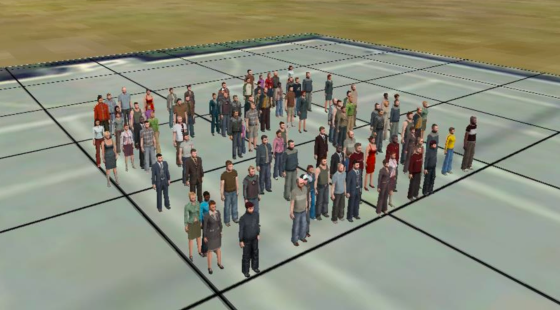
\includegraphics[width=\textwidth]{Pictures/Figures/Los/A.png}
    \caption*{\textbf{A} (0-1 person/m\textsuperscript{2}). Head, shoulders, chest, and feet are visible.}
  \end{subfigure}%
  \hspace{0.06\textwidth}
  \begin{subfigure}[t]{0.45\textwidth}
    \centering
    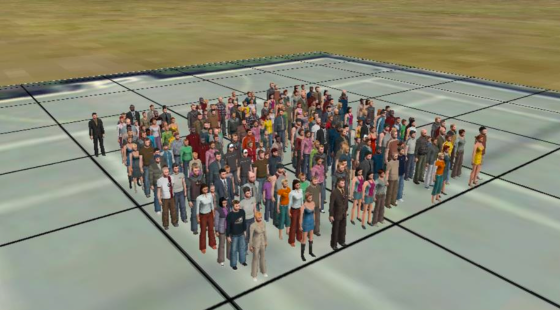
\includegraphics[width=\textwidth]{Pictures/Figures/Los/B.png}
    \caption*{\textbf{B} (1-2 people/m\textsuperscript{2}). Head, shoulders, chest, and feet are visible.}
  \end{subfigure}

  \begin{subfigure}[t]{0.45\textwidth}
    \centering
    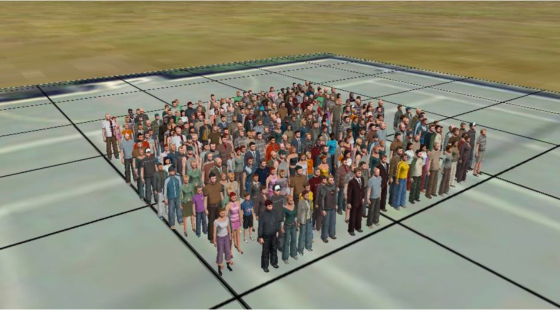
\includegraphics[width=\textwidth]{Pictures/Figures/Los/C.png}
    \caption*{\textbf{C} (2-3 people/m\textsuperscript{2}). Head, shoulders, and chest are visible.}
  \end{subfigure}%
  \hspace{0.06\textwidth}
  \begin{subfigure}[t]{0.45\textwidth}
    \centering
    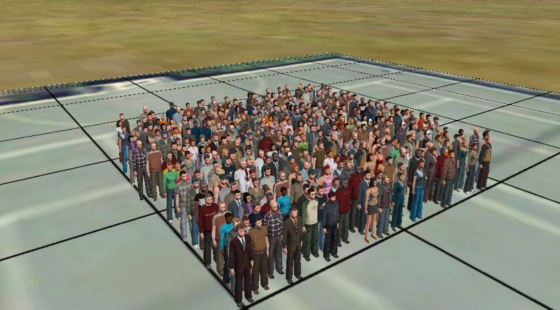
\includegraphics[width=\textwidth]{Pictures/Figures/Los/D.png}
    \caption*{\textbf{D} (3-4 people/m\textsuperscript{2}). Head, shoulders, and chest are visible.}
  \end{subfigure}

  \begin{subfigure}[t]{0.45\textwidth}
    \centering
    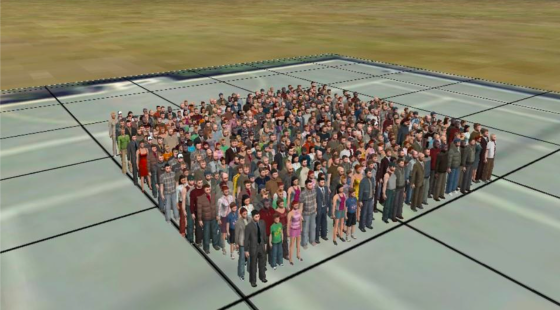
\includegraphics[width=\textwidth]{Pictures/Figures/Los/E.png}
    \caption*{\textbf{E} (4-5 people/m\textsuperscript{2}). Head and shoulders are visible.}
  \end{subfigure}%
  \hspace{0.06\textwidth}
  \begin{subfigure}[t]{0.45\textwidth}
    \centering
    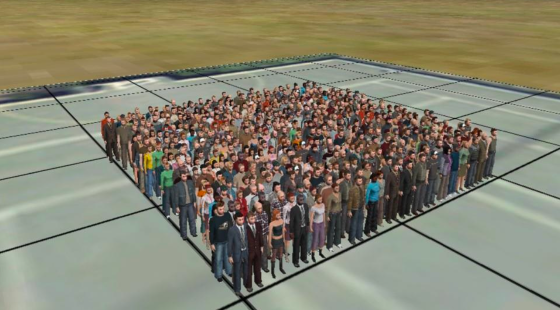
\includegraphics[width=\textwidth]{Pictures/Figures/Los/F.png}
    \caption*{\textbf{F} (5+ people/m\textsuperscript{2}). Only heads are visible.}
  \end{subfigure}
  \caption{Roskilde Festival's internal implementation of Levels of Service (LoS), using a scale of A-F. The images serve as visual examples of the different LoS levels, used to estimate crowd density on-site or through video footage. Roskilde relies on visual cues, namely the visibility of heads, shoulders, and feet, to assess crowd density.}
  \label{fig:fruin}
\end{figure}

\subsection{Key metrics}
\label{sec:key-metrics}



Given the workflows outlined above, we can identify the following key metrics that Roskilde Festival relies on to assess crowd safety:

\begin{itemize}
  \item \textbf{Ingress/Egress Counts}: The number of people entering (ingress) or leaving (egress) a monitored area.
  \item \textbf{Flow Rates}: The rate at which people enter or exit an area over specific time periods (e.g., per minute, per hour), including net change and peak rates.
  \item \textbf{Cumulative Counts}: A running total showing the net number of individuals within the monitored area over time.
  \item \textbf{Crowd Density}: The concentration of people within an area, typically expressed as people per square meter (people/m\textsuperscript{2}).
  \item \textbf{Movement Patterns}: The general paths, directions, origins, and destinations of people moving within the monitored space.
\end{itemize}

\subsection{Revisiting the problem definition}
As outlined in the previous sections, Roskilde Festival currently utilizes established frameworks and workflows for proactive crowd safety management. Their approach demonstrates a commitment to data-driven planning and analysis. However, a significant challenge lies not in the \textit{analysis} of data, but in the \textit{acquisition} of reliable and objective data. While the festival's safety team already has the tools necessary to interpret and act upon key metrics, the current means of gathering this information often rely on manual, time-consuming, or subjective methods.

A prime example is the assessment of ingress/egress flow rates. As described by Mads Therkildsen, Safety Lead at Roskilde Festival, a common practice involves manually counting individuals passing through an entrance for a short period, such as one or two minutes, and then extrapolating this count to estimate hourly flow (Appendix \ref{appendix:rf-feb-25}). While practical, this method provides only partial data and is likely inaccurate, especially during rapidly changing conditions. Similarly, crowd density is currently gauged primarily through subjective visual assessment using an internal Levels of Service (LoS) scale, as illustrated in Figure \ref{fig:fruin}. The current process relies on observers estimating density based on visual cues like the visibility of heads, shoulders, and feet. Consequently, the true density value across different areas and times remains largely unknown.

These examples highlight the core limitation: the absence of an efficient system to autonomously and objectively gather quantitative data on key crowd metrics. As Roskilde Festival already employs a data-driven approach to crowd safety management, such a system would integrate directly into their existing workflows. The following sections explore potential technical solutions to solve this challenge, eventually proposing a product.

\section{Comparing technical solutions}

\subsection{Global Positioning System (GPS)}
\label{sec:gps}

Using GPS to track the location of festival-goers is a common practice, and likely the easiest to implement technology in this comparison. This is typically achieved by providing guests with a mobile app that uses their smartphone's GPS to track their location. Of course, this requires the guests to opt in to location tracking, as well as there being a sufficient reason for doing so. In almost all cases, this is attempted by including a map of the festival in the app, as visible in Figure \ref{fig:festival_apps}. This feature, however, still functions without location tracking, and therefore doesn't guarantee users will grant data access. Even before this obstacle is met, there is the question of whether festival-goers will actually use the app. A study on Roskilde Festival 2015 by the Copenhagen Business School  found that of the 60 thousand people who installed the festival application, 44 thousand opted-in to allowing anonymous tracking; yielding 38.678 unique users who were present inside the festival area \cite{rf_app}. This equates to slightly under 30\% of the total 130 thousand attendees. In a crowd safety context, this is a significant limitation, as the location data gathered is not representative of entire crowds.

\begin{figure}
  \centering
  \begin{subfigure}{.3\textwidth}
    \centering
    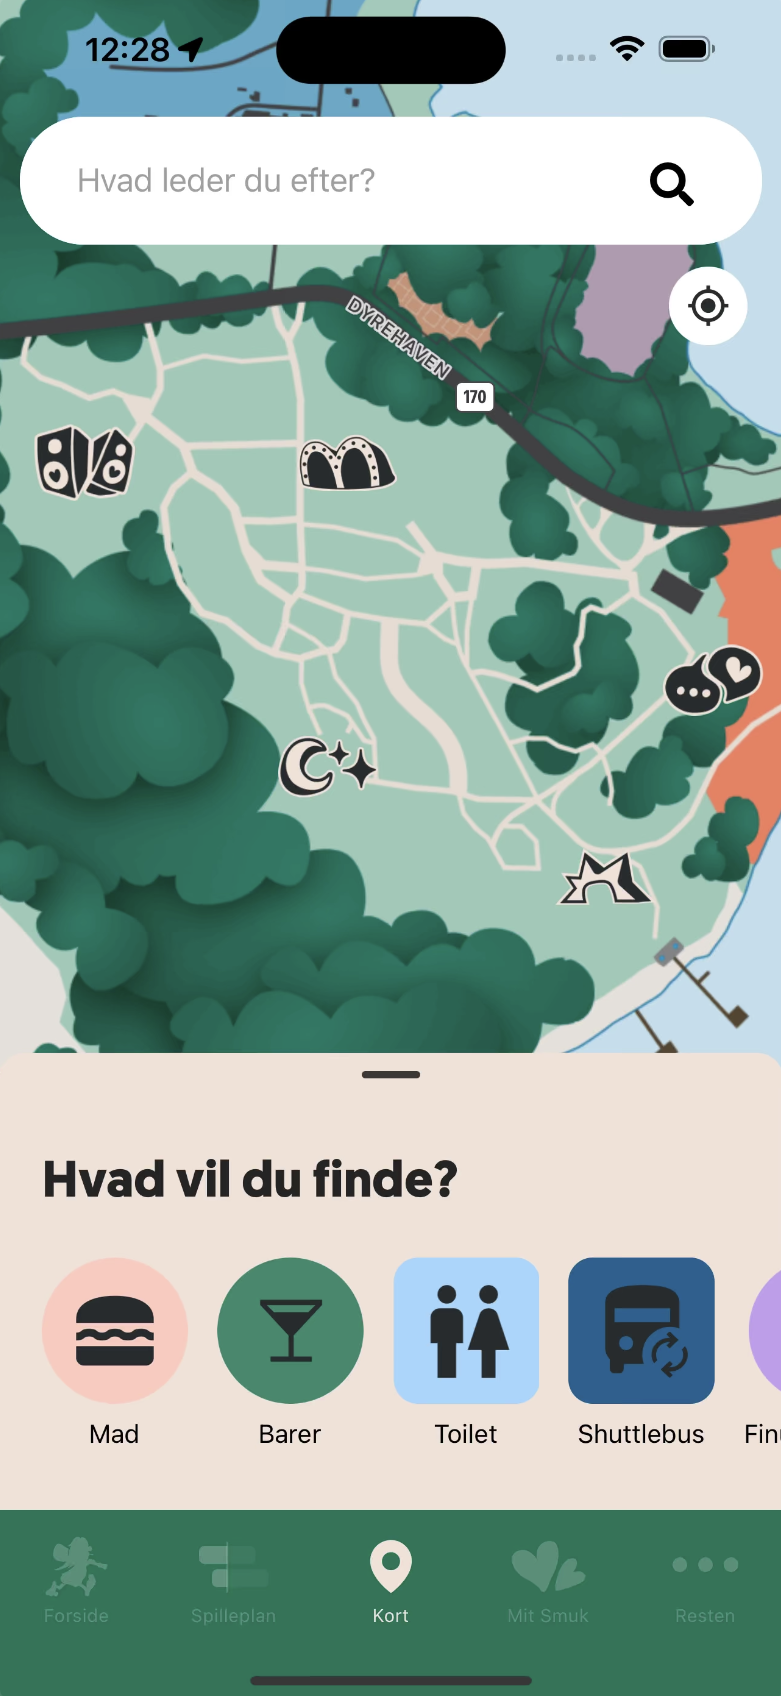
\includegraphics[width=4cm]{Pictures/Misc/smukfest_app.png}
    \caption{Smukfest app \cite{smukfest_app}}
    \label{fig:smukfest_app}
  \end{subfigure}%
  \begin{subfigure}{.3\textwidth}
    \centering
    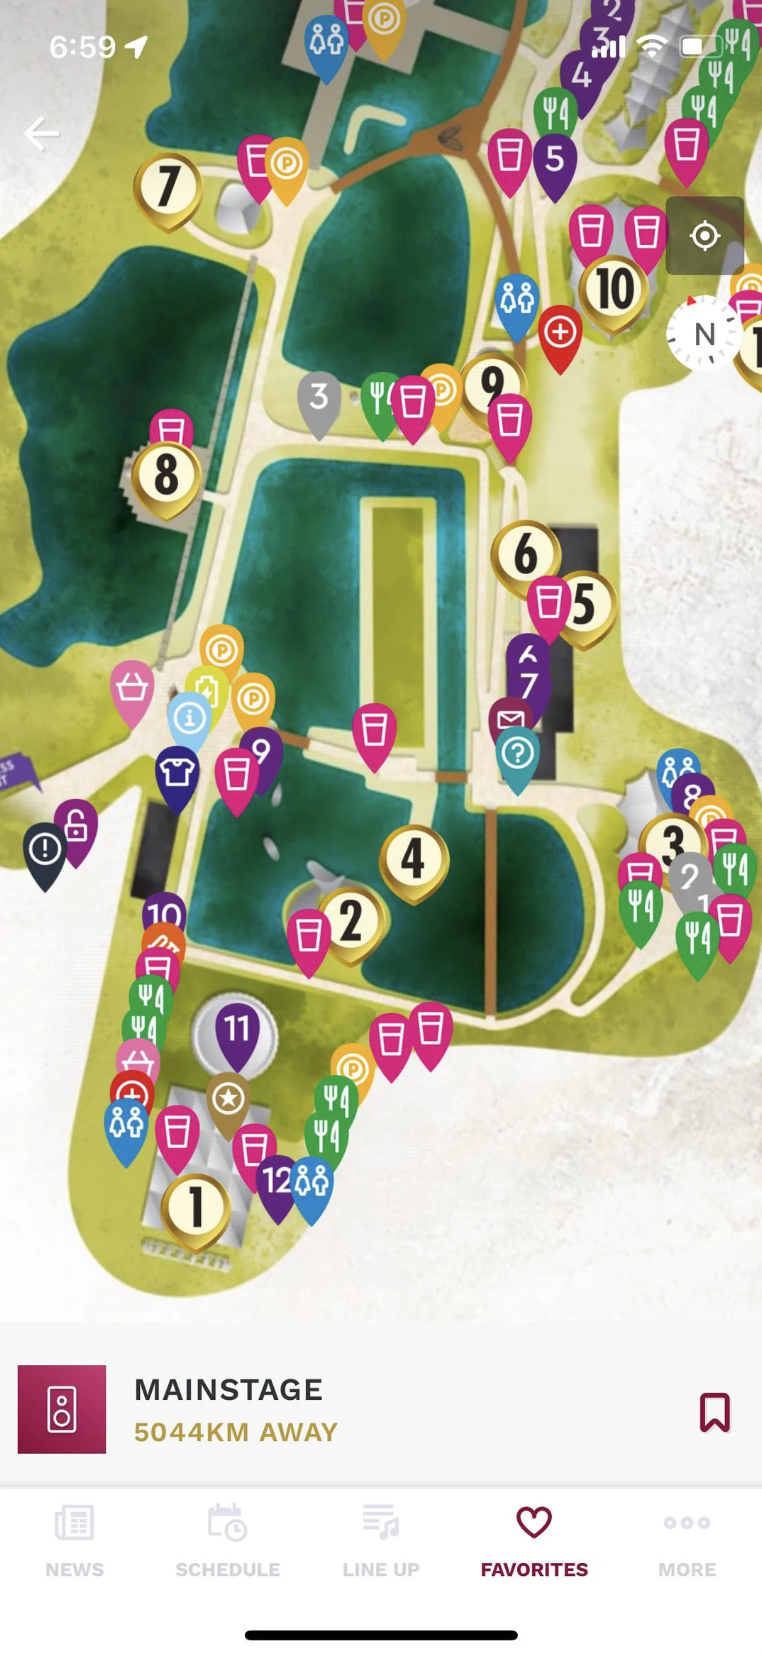
\includegraphics[width=4cm]{Pictures/Misc/tomorrowland_app.png}
    \caption{Tomorrowland app \cite{tomorrowland_app}}
    \label{fig:tomorrowland_app}
  \end{subfigure}
  \begin{subfigure}{.3\textwidth}
    \centering
    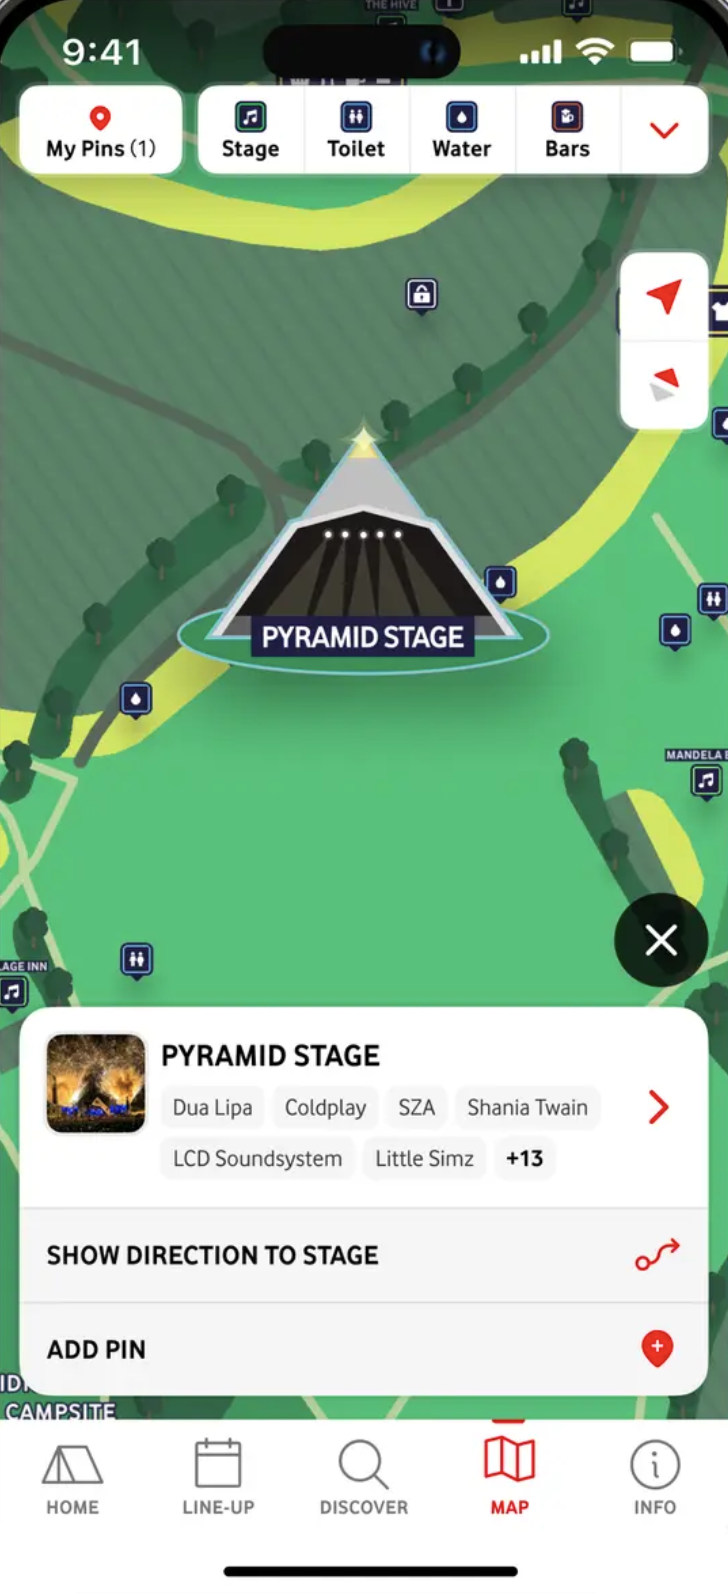
\includegraphics[width=4cm]{Pictures/Misc/glastonbury_app.png}
    \caption{Glastonbury app \cite{glastonbury_app}}
    \label{fig:glastonbury_app}
  \end{subfigure}
  \caption{Examples of map features in music festival mobile apps (Smukfest, Tomorrowland, Glastonbury), often used to encourage attendees to enable GPS location tracking.}
  \label{fig:festival_apps}
\end{figure}


Beyond low adoption and potential privacy concerns, the technical limitations of GPS also hinder its utility for detailed crowd analysis. According to GPS.gov, GPS-enabled smartphones are typically accurate only to within a 4.9-meter radius under open sky; however, their accuracy worsens near buildings, bridges, and trees \cite{gps}. While a 4.9-meter radius might seem acceptable for general location awareness on a festival map, this level of uncertainty significantly hinders the calculation of precise crowd dynamics metrics. Furthermore, the degradation of accuracy near structures is particularly problematic in festival environments, which often feature large stages, tents, and temporary structures -- precisely where accurate monitoring is most needed. The effectiveness of GPS tracking is also contingent on factors outside the organizers' control, such as users keeping their phones charged and maintaining a stable mobile data connection.

Compared to infrastructure-based monitoring systems (like cameras or dedicated sensors), GPS relies heavily on user cooperation and device functionality, making it less suitable for generating the consistent, high-resolution data needed for proactive crowd safety management and detailed post-event analysis. Therefore, while mobile app GPS data can offer some high-level insights into general attendee distribution, its inherent limitations in accuracy make it insufficient as a primary tool for gathering crowd dynamics measurements.

\subsection{Bluetooth beacons}
Another potential solution for gathering crowd dynamics data involves utilizing Bluetooth Low Energy (BLE), a wireless communication technology designed for low power consumption. This technology is typically utilized in Bluetooth beacons -- devices that periodically transmit signals that can be detected by nearby receivers, such as smartphones or dedicated hardware. These signals can be used to determine the proximity of beacons to the receivers, as well as location estimation through triangulation techniques, requiring three or more receivers. This capability is increasingly utilized for proximity marketing, indoor navigation, and positional tracking, typically in retail environments \cite{bt_beacon}. It has also been effectively used for guest tracking in environments like museums, as demonstrated in a study at the Galleria Borghese, where visitors were given portable BLE beacons tracked by fixed receivers \cite{borghese}.

Finding examples of BLE beacons utilized at large outdoor events is more challenging, as the technology has its own set of drawbacks. Similar to GPS-based mobile apps, the effectiveness of Bluetooth beacon systems is significantly contingent on user cooperation. Beacons can be implemented either as dedicated physical devices or embedded within smartphone applications. The latter is simpler and cheaper, however motiving users to install an app is challenging, as discussed in section \ref{sec:gps}. The former approach has challenges of its own, as requiring event participants to carry a dedicated device demands a value proposition of its own, not to mention the overhead costs involved in developing, deploying, and maintaining the system. Given that beacon signals have an effective range of 30 meters without obstructions, a considerable number of receivers are necessary to ensure adequate coverage \cite{bt_beacon}.

Ultimately, the most critical factor for crowd dynamics analysis is the technology's accuracy. A study conducted at a large exhibition in Japan evaluated the accuracy of trajectory estimation using Bluetooth beacons. They found that  in 68\% of instances, their positional estimates were accurate within a radius of 18 meters \cite{bt_japan}. While still useful for certain applications like indoor tracking or general zone classification, this level of accuracy is significantly less precise than typically achievable with GPS (Section \ref{sec:gps}). This limitation, combined with the dependency on user adoption and implementation costs, makes Bluetooth beacons a less favorable option for gathering crowd dynamics data at large outdoor events.

\subsection{Camera solutions}
Camera-based solutions leverage existing CCTV systems in conjunction with computer vision algorithms to analyze crowd dynamics. Utilizing video footage from these camera systems, novel advancements in machine learning and computer vision enable automated extraction of valuable metrics.

A primary advantage of this approach compared to GPS (Section 2.3.1) and Bluetooth beacon (Section 2.3.2) systems is its independence from attendee cooperation. Unlike solutions requiring festival-goers to install an app, enable location services, carry a specific device, or keep their phones charged, camera-based analysis operates passively. It gathers data from anyone within the camera's field of view, potentially offering a more comprehensive and unbiased view of crowd behavior across monitored areas. This circumvents the significant limitations associated with low adoption rates and opt-in requirements inherent in user-device-dependent methods.

(competitor analysis)

\section{Proposed solution}
\label{sec:solution}

% also state which areas will be monitored and analyzed

\section{Legal Feasibility}
\label{sec:legal-feasibility}
When dealing with CCTV footage, there are a number of legal considerations to take into account. This section outlines the primary legal considerations for the project, focusing on Danish CCTV law, the General Data Protection Regulation (GDPR), and the EU AI Act. As this section focuses on the legal feasibility of the product itself, the theoretical administrator will be referred to as Fluxense, the startup mentioned in Section \ref{sec:fluxense}. This name was also used in the Non-Disclosure Agreement (NDA) signed with Roskilde Festival, which underscores the importance of data confidentiality and adherence to applicable laws.

The Danish Act on CCTV Surveillance (tv-overvågningsloven) regulates the use of surveillance cameras in Denmark, which is evidently relevant to this project. The Act generally prohibits private individuals and organizations from conducting surveillance in public areas of "general traffic," such as streets and squares \cite{cctv_law}. In the context of Roskilde Festival, however, this legislation does not apply, as it is not considered a public area. In these cases, the Act refers to data protection legislation, as outlined by The Danish Data Protection Agency (DDPA) and the European Union's GDPR. GDPR establishes a comprehensive framework for protecting individuals' privacy and personal data, including CCTV footage. Both the DDPA and GDPR present two critical roles: the data controller and the data processor. The data controller is the entity that determines the purposes and means of processing personal data, while the data processor is responsible for processing data on behalf of the controller \cite{gdpr_dpa}. Both roles are formally defined in a data processing agreement (DPA) between the two parties. In this case, Roskilde Festival acts as the data controller, while Fluxense is the data processor. As data processor, Fluxense is responsible for ensuring that all data processing activities comply with GDPR regulations. This includes ensuring secure processing, containment of sensitve data, as well as prompt deletion of data at the request of the data controller (GDPR Article 28 \cite{gdpr_article_28}).

The EU AI Act establishes a regulatory framework for artificial intelligence systems based on a risk-based approach, which is relevant to the AI-enabled video analytics central to this project. The legislation entered into force on August 1, 2024, and will be applicable in stages over the coming months and years \cite{ai_act_passed}. The Act classifies AI systems into four risk categories: unacceptable risk, high risk, limited risk, and minimal risk. As documentation pertaining to the explicit categorization criteria will not be available until August 2026, it is difficult to speculate on the risk classification of the proposed system. Most relevantly, however, the Act is not applicable within research, testing or development, as is the focus of this project.
